\documentclass{beamer}
\usetheme{metropolis}
\usepackage{graphicx}
\usepackage{subfig}
\title{Calculus-Based Physics-1: Mechanics (PHYS150-01): Week 3}
\date{September 18th - September 22nd, 2017}
\author{Jordan Hanson}
\institute{Whittier College Department of Physics and Astronomy}

\begin{document}
\maketitle

\section{Week 2 Review}

\begin{frame}{Week 2 Review}
\begin{enumerate}
\item Displacement, and instantaneous velocity and acceleration
\begin{itemize}
\item \textit{Mathematics review}: taking derivatives
\item Average velocity and average acceleration
\end{itemize}
\item The case of constant acceleration
\begin{itemize}
\item An \textit{an equation of motion} for constant acceleration
\item Derivation of \alert{common equations of motion}
\item Average quantities and exercises
\end{itemize}
\item \textbf{Lab Activity: Measuring acceleration of gravity: \textit{g}}
\item Exercises with vectors, graphs, and equations of motion
\end{enumerate}
\end{frame}

\section{Week 2 Review Problems}

\begin{frame}{Week 2 Review Problems}
\small
\begin{minipage}[b]{0.45\linewidth}
If a subway train is moving to the left (has a negative velocity) and then comes to a stop, what is the direction of its acceleration? Is the acceleration positive or negative?
\begin{itemize}
\vspace{0.5cm}
\item A: To the right, positive
\item B: To the right, negative
\item C: To the left, positive
\item D: To the left, negative
\end{itemize}
\end{minipage}
\hspace{0.5cm}
\begin{minipage}[b]{0.45\linewidth}
An object that is thrown straight up falls back to Earth.  When is its velocity zero?  Does its velocity change direction?  Does the acceleration change sign?
\begin{itemize}
\item During flight, yes, no
\item At the peak height, yes, yes
\item At the peak height, yes, no
\item During flight, no, no
\end{itemize}
\end{minipage}
\end{frame}

\section{Week 3 Summary}

\begin{frame}{Week 3 Summary}
\begin{enumerate}
\item Displacement, velocity and acceleration vectors \alert{as functions of time}
\begin{itemize}
\item Breaking into components
\item Derivatives of components
\end{itemize}
\item Combining free-fall and vector components: \alert{projectile motion}
\begin{itemize}
\item The independence of velocity components
\item \textbf{Lab-activity: testing component independence}
\end{itemize}
\item Relative motion and reference frames
\begin{itemize}
\item Relative motion in one-dimension
\item Relative motion in two-dimensions
\end{itemize}
\end{enumerate}
\end{frame}

\section{Vectors as functions of time}

\begin{frame}{Vectors as functions of time}
In general, the displacement of an object depends on time:
\begin{equation}
\vec{r}(t) = x(t) \hat{i} + y(t) \hat{j} + z(t) \hat{k}
\end{equation}
\begin{itemize}
\item $x(t)$ is the displacement in the x-direction
\item $y(t)$ is the displacement in the y-direction
\item $z(t)$ is the displacement in the z-direction
\end{itemize}
\end{frame}

\begin{frame}{Vectors as functions of time}
\begin{figure}
\centering
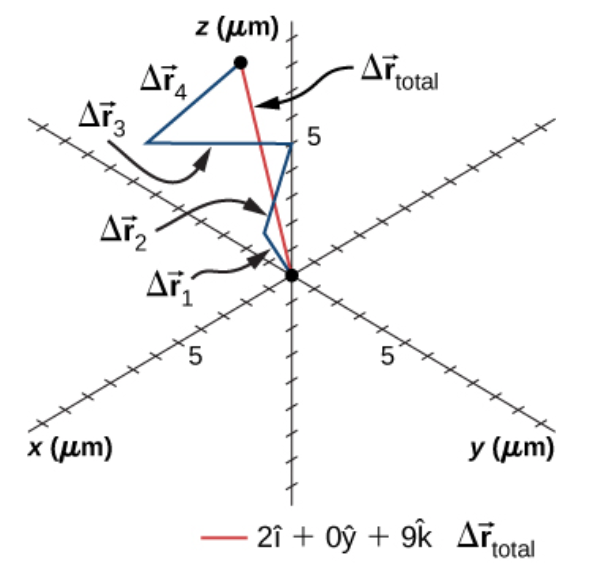
\includegraphics[width=0.6\textwidth,trim=0cm 2cm 0cm 0cm,clip=true]{figures/Brownian.png}
\caption{\label{fig:brown} An example of a displacement vector at different moments in time.}
\end{figure}
\end{frame}

\begin{frame}{Vectors as functions of time}
The particle in Fig. \ref{fig:brown} has four displacement vectors at four moments in time:
\begin{itemize}
\item $\vec{r}_{\rm 1} = 2.0\hat{i} + 1.0\hat{j} + 3.0\hat{k}\quad(\mu m)$ at $t_{\rm 1}$
\item $\vec{r}_{\rm 2} = -1.0\hat{i} + 0.0\hat{j} + 3.0\hat{k}\quad(\mu m)$ at $t_{\rm 2}$
\item $\vec{r}_{\rm 3} = 4.0\hat{i} + -2.0\hat{j} + 1.0\hat{k}\quad(\mu m)$ at $t_{\rm 3}$
\item $\vec{r}_{\rm 4} = -3.0\hat{i} + 1.0\hat{j} + 2.0\hat{k}\quad(\mu m)$ at $t_{\rm 4}$
\end{itemize}
What is the total displacement of the particle from the origin?
\end{frame}

\begin{frame}{Vectors as functions of time}
We can think of this type of problem as an accounting problem, lining up columns (units: $\mu m$):
\begin{figure}
\begin{tabular}{| c | c | c | c | c |}
\hline
$t_{\rm i}$ & $\vec{r}_{\rm i}(t_{\rm i})$ & $x(t_{\rm i})$ & $y(t_{\rm i})$ & $y(t_{\rm i})$ \\
\hline
$t_{\rm 1}$ & $\vec{r}_{\rm 1}(t_{\rm 1})$ & 2.0 & 1.0 & 3.0 \\
\hline
$t_{\rm 2}$ & $\vec{r}_{\rm 2}(t_{\rm 2})$ & -1.0 & 0.0 & 3.0 \\
\hline
$t_{\rm 3}$ & $\vec{r}_{\rm 3}(t_{\rm 3})$ & 4.0 & -2.0 & 1.0 \\
\hline
$t_{\rm 4}$ & $\vec{r}_{\rm 4}(t_{\rm 4})$ & -3.0 & 1.0 & 2.0 \\
\hline
\hline
$t_{\rm total}$ & $\vec{r}_{\rm total}(t_{\rm total})$ & 2.0 & 0.0 & 9.0 \\
\hline
\end{tabular}
\caption{\label{tab:account} Accounting for the different displacement components, in units of $\mu m$.}
\end{figure}
\end{frame}

\begin{frame}{Vectors as functions of time}
\begin{figure}
\centering
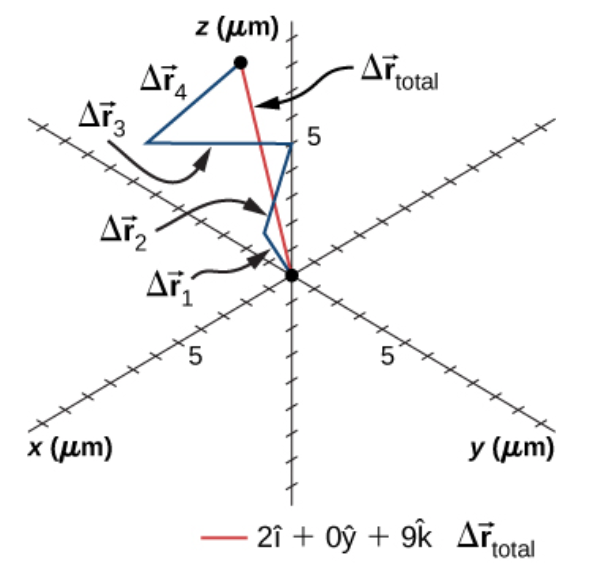
\includegraphics[width=0.6\textwidth]{figures/Brownian.png}
\caption{\label{fig:brown2} The total displacement of the particle is $\vec{r}_{\rm total} = 2.0\hat{i} + 0.0\hat{k} + 9.0\hat{k}\quad (\mu m)$.}
\end{figure}
\end{frame}

\begin{frame}{Vectors as functions of time}
\small
The 18th hole at Pebble Beach Golf Course is a dogleg to the left of length 496.0 meters.  The fairway off the tee is taken to be the x direction.  A golfer hits his tee shot a distance of 300 meters, corresponding to a displacement of $\vec{r}_{\rm 1} = 300.0 \hat{i} \quad (m)$, and then hits a second shot 189.0 meters with $\vec{r}_{\rm 2} = 172.0 \hat{i} + 80.3 \hat{j} \quad m$.  What is the final displacement from the tee?
\begin{itemize}
\item $\vec{r}_{\rm final} = 172.0 \hat{i} + 80.3\hat{j}\quad (m)$
\item $\vec{r}_{\rm final} = 172.0 \hat{i} + 380.3\hat{j}\quad (m)$
\item $\vec{r}_{\rm final} = 472.0 \hat{i} + 0.0\hat{j}\quad (m)$
\item $\vec{r}_{\rm final} = 472.0 \hat{i} + 80.3\hat{j}\quad (m)$
\end{itemize}
\end{frame}

\begin{frame}{Vectors as functions of time}
\small
If the first shot takes 5.0 seconds, the second shot takes 4.0 seconds, and the walking time in between the shots is 60.0 seconds, what is the average velocity vector for the ball after the two shots?
\begin{itemize}
\item $\vec{r}_{\rm final} = 1.7 \hat{i} + 8.3\hat{j}\quad (m/s)$
\item $\vec{v}_{\rm final} = 172.0 \hat{i} + 80.3\hat{j}\quad (m/s)$
\item $\vec{v}_{\rm final} = 6.8 \hat{i} + 1.2\hat{j}\quad (m)$
\item $\vec{v}_{\rm final} = 6.8 \hat{i} + 1.2\hat{j}\quad (m/s)$
\end{itemize}
\end{frame}

\begin{frame}{Vectors as functions of time}
The prior problem indicates something you may already have guessed:
\begin{equation}
\vec{v}_{\rm avg}(t) = v_{\rm x}(t) \hat{i} + v_{\rm y}(t) \hat{j} + v_{\rm z}(t) \hat{k} = \frac{\Delta\vec{r}}{\Delta t}
\end{equation}
\begin{itemize}
\item $v_{\rm x}(t)$ is the velocity in the x-direction
\item $v_{\rm y}(t)$ is the velocity in the y-direction
\item $v_{\rm z}(t)$ is the velocity in the z-direction
\end{itemize}
In other words, we divide each displacement component by the time, to get a vector where each component is the average velocity in that direction.  $\Delta\vec{r} = \vec{r}_{\rm f} - \vec{r}_{\rm i}$.
\end{frame}

\section{Answers}

\begin{frame}{Answers}
\begin{columns}[T]
\begin{column}{0.5\textwidth}
\begin{itemize}
\item To the right, positive
\item At the peak height, yes, yes
\item $\vec{r}_{\rm final} = 472.0 \hat{i} + 80.3\hat{j}\quad (m)$
\item $\vec{v}_{\rm final} = 6.8 \hat{i} + 1.2\hat{j}\quad (m/s)$
\end{itemize}
\end{column}
\begin{column}{0.5\textwidth}
\begin{itemize}
\item 
\end{itemize}
\end{column}
\end{columns}
\end{frame}

\end{document}
